\documentclass[conference]{IEEEtran}
\IEEEoverridecommandlockouts
% The preceding line is only needed to identify funding in the first footnote. If that is unneeded, please comment it out.
\usepackage{cite}
\usepackage{amsmath,amssymb,amsfonts}
\usepackage{algorithmic}
\usepackage{graphicx}
\usepackage{textcomp}
\usepackage{xcolor}
\usepackage{float}
\usepackage{caption}
\usepackage{amsmath}
\usepackage{tikz}
\def\BibTeX{{\rm B\kern-.05em{\sc i\kern-.025em b}\kern-.08em
    T\kern-.1667em\lower.7ex\hbox{E}\kern-.125emX}}
\begin{document}

\newcommand{\RN}[1]{%
  \textup{\uppercase\expandafter{\romannumeral#1}}%
}

\title{CENG 435 - Data Communications and Networking\\
Term Project - Part \RN{1}}

\author{\IEEEauthorblockN{Sina Sehlaver}
\IEEEauthorblockA{2099729}
\and
\IEEEauthorblockN{Beyazit Yalcinkaya}
\IEEEauthorblockA{2172138}
}

\maketitle

%\begin{abstract}
%abcd
%\end{abstract}

%\begin{IEEEkeywords}
%component, formatting, style, styling, insert
%\end{IEEEkeywords}

\section{Introduction}

\section{Methodology}

\section{Implementation}

\section{Experimental Results}

\section{Conclusion}

\begin{figure}[H]
\caption{Topology with Link Costs}
	\centering
	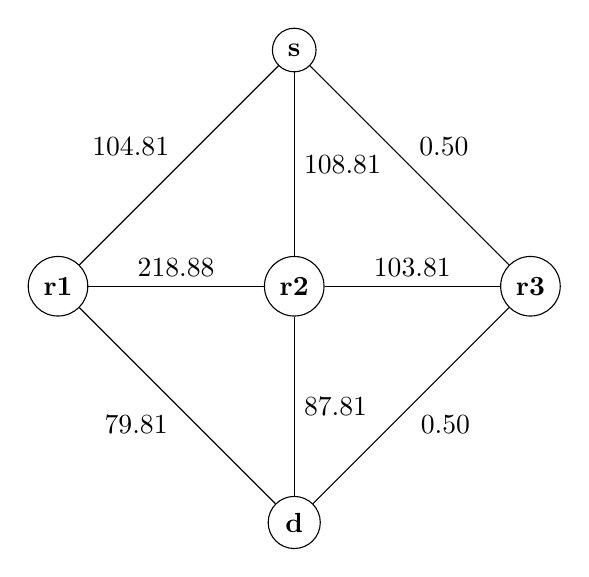
\begin{tikzpicture}
	\node[shape=circle,draw=black] (s) at (2, 4) {\textbf{s}};
	\node[shape=circle,draw=black] (r1) at (-1, 1) {\textbf{r1}};
	\node[shape=circle,draw=black] (r2) at (2, 1) {\textbf{r2}};
	\node[shape=circle,draw=black] (r3) at (5, 1) {\textbf{r3}};
	\node[shape=circle,draw=black] (d) at (2, -2) {\textbf{d}};
	\path[-] (r1) edge  node[above left] {104.81} (s);
	\path[-] (r1) edge  node[below left] {79.81} (d);
	\path[-] (r2) edge  node[above] {218.88} (r1);
	\path[-] (r2) edge  node[above] {103.81} (r3);
	\path[-] (r2) edge  node[right] {108.81} (s);
	\path[-] (r2) edge  node[right] {87.81} (d);
	\path[-] (r3) edge  node[above right] {0.50} (s);
	\path[-] (r3) edge  node[below right] {0.50} (d);
	\end{tikzpicture} 
\end{figure}


\begin{table}[H]
\centering
\caption{Initial}
\label{my-label1}
\begin{tabular}{|c|c|c|}
\hline
\textbf{Node}&\textbf{Distance from s}&\textbf{Previous node}\\ \hline
s&$0$&None\\ \hline
r1&$\infty$&None\\ \hline
r2&$\infty$&None\\ \hline
r3&$\infty$&None\\ \hline
d&$\infty$&None\\ \hline
\end{tabular}
\end{table}


\begin{table}[H]
\centering
\caption{After First Iteration}
\label{my-label1}
\begin{tabular}{|c|c|c|}
\hline
\textbf{Node}&\textbf{Distance from s}&\textbf{Previous node}\\ \hline
s&$0$&None\\ \hline
r1&$104.81$&s\\ \hline
r2&$108.81$&s\\ \hline
r3&$0.50$&s\\ \hline
d&$\infty$&None\\ \hline
\end{tabular}
\end{table}


\begin{table}[H]
\centering
\caption{After Second Iteration}
\label{my-label1}
\begin{tabular}{|c|c|c|}
\hline
\textbf{Node}&\textbf{Distance from s}&\textbf{Previous node}\\ \hline
s&$0$&None\\ \hline
r1&$104.81$&s\\ \hline
r2&$104.31$&r3\\ \hline
r3&$0.50$&s\\ \hline
d&$1.00$&r3\\ \hline
\end{tabular}
\end{table}


\begin{table}[H]
\centering
\caption{After Third Iteration}
\label{my-label1}
\begin{tabular}{|c|c|c|}
\hline
\textbf{Node}&\textbf{Distance from s}&\textbf{Previous node}\\ \hline
s&$0$&None\\ \hline
r1&$80.81$&d\\ \hline
r2&$88.81$&d\\ \hline
r3&$0.50$&s\\ \hline
d&$1.00$&r3\\ \hline
\end{tabular}
\end{table}



\begin{figure*}[t]
\caption{Mean End-to-End Delay vs Network Emulated Delay}
\centerline{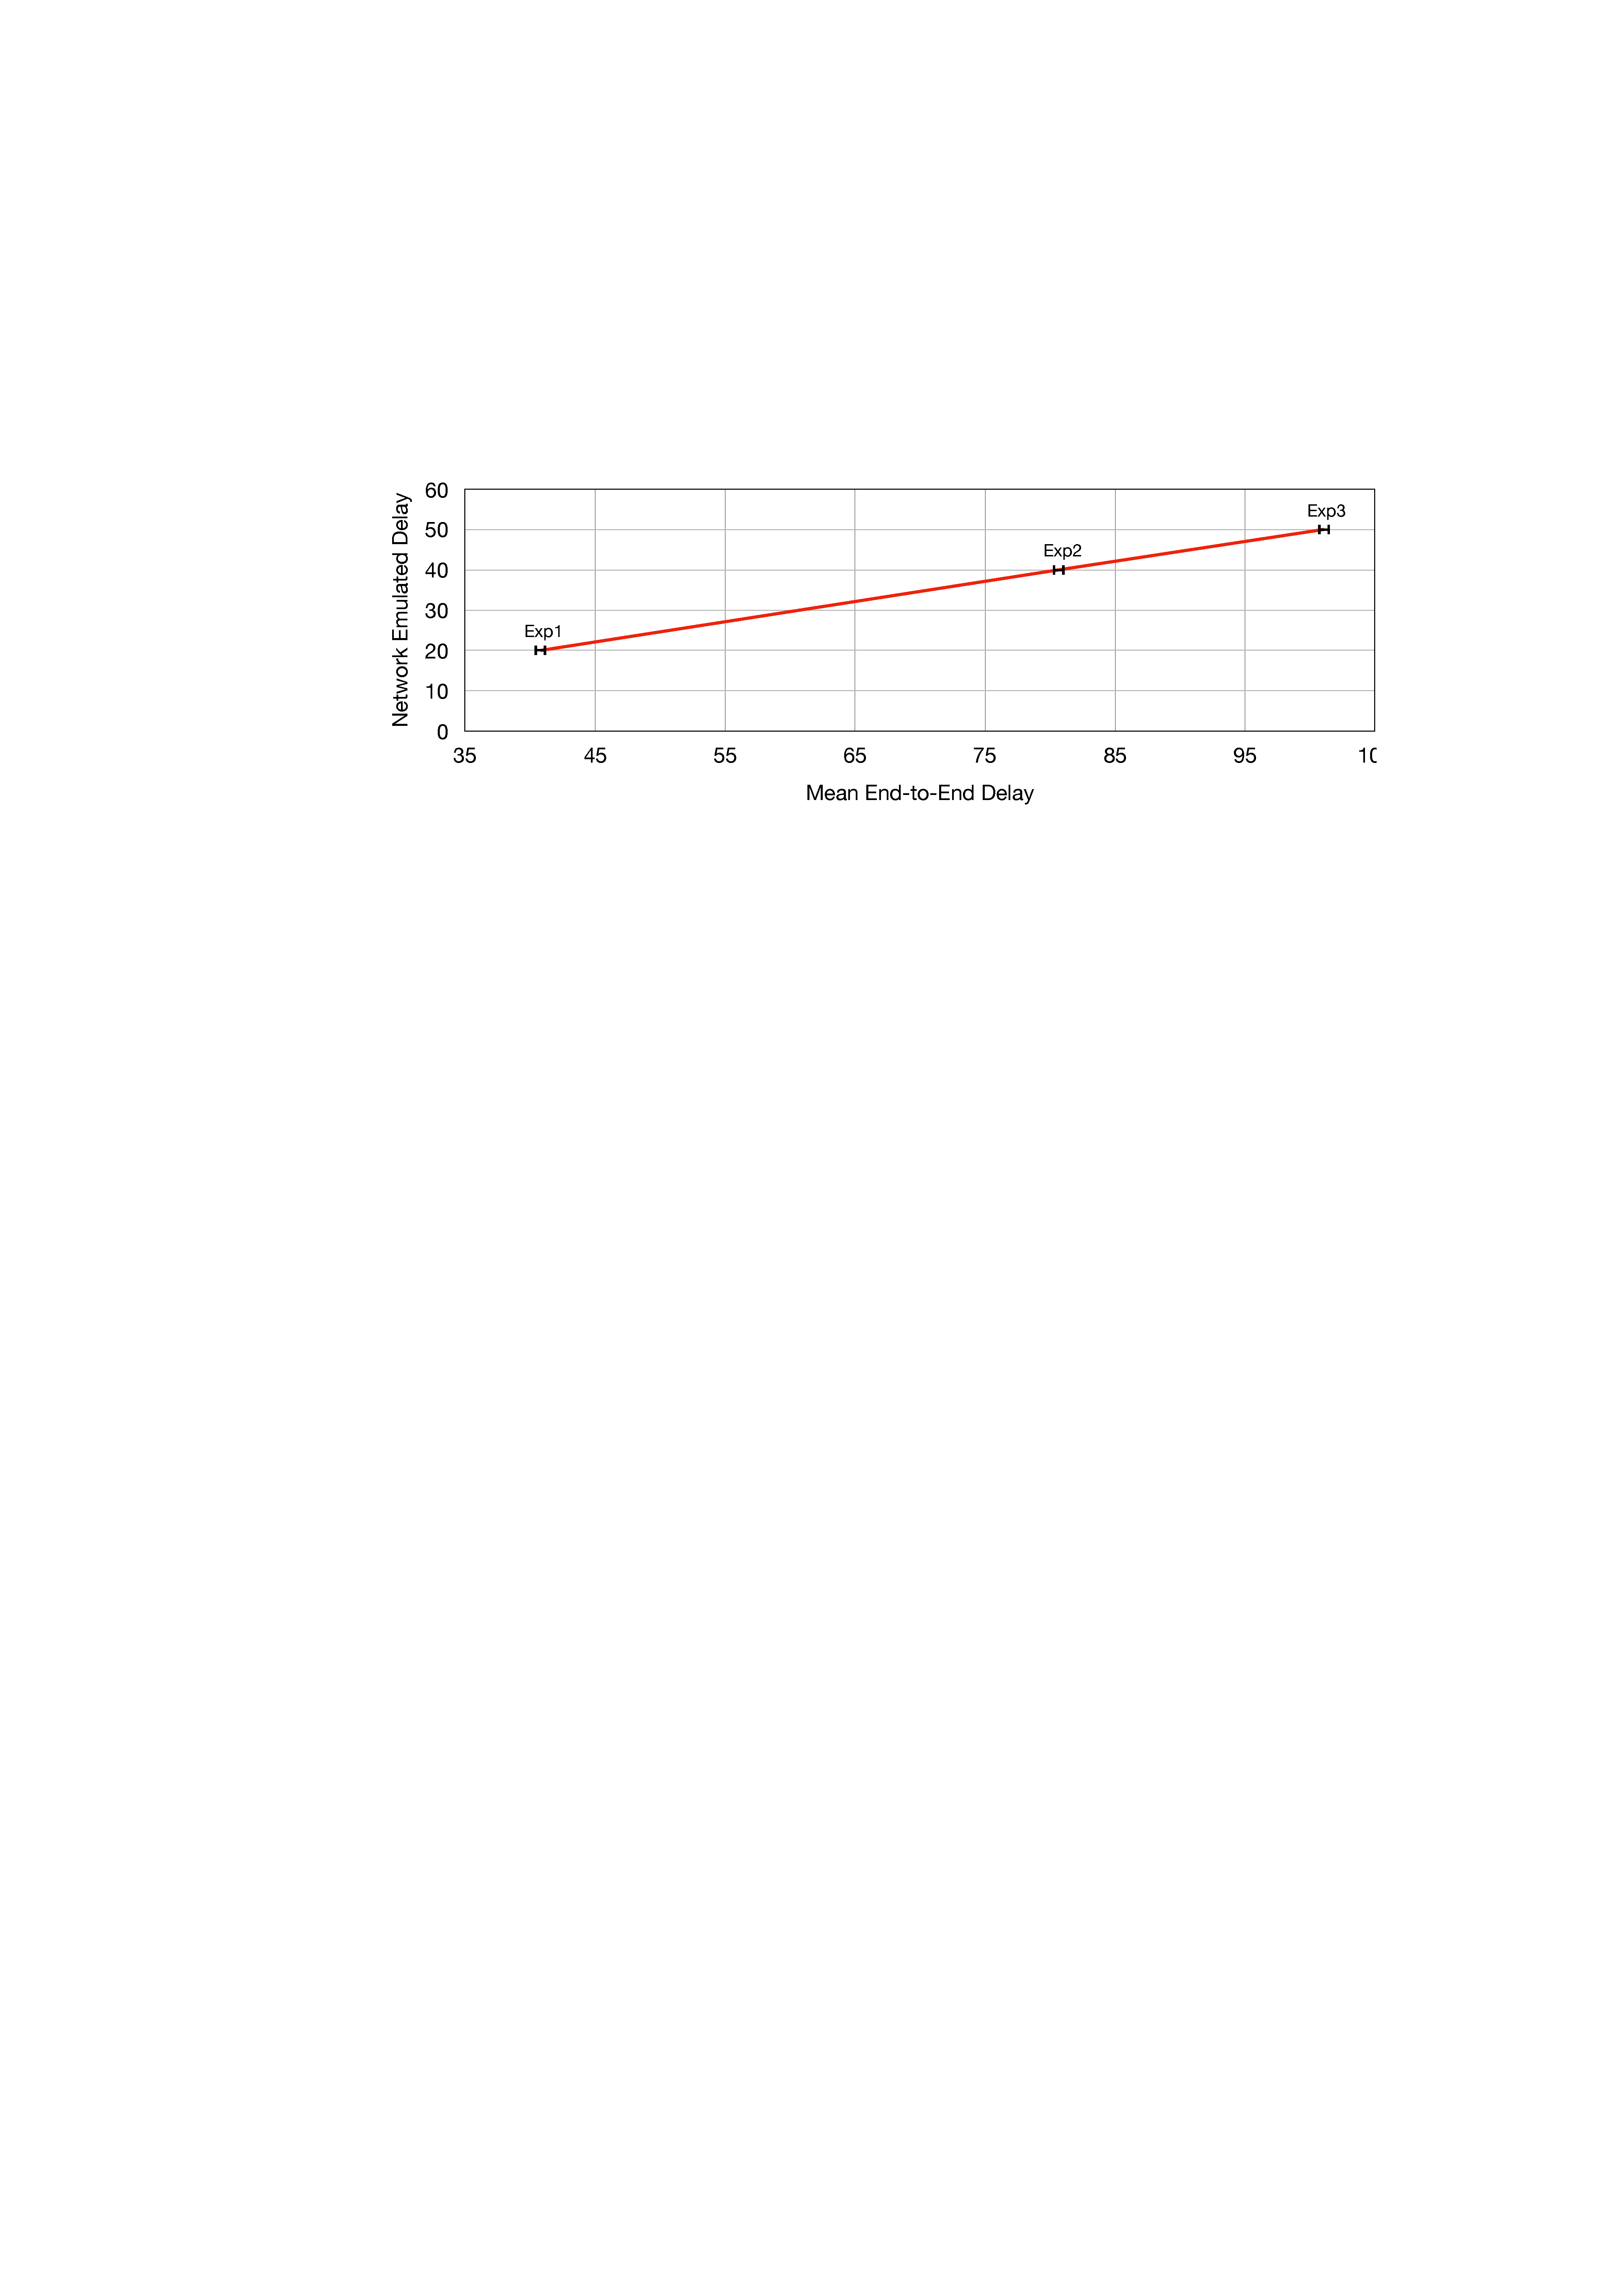
\includegraphics[width=\textwidth]{exps.pdf}}
\label{fig}
\end{figure*}




%\begin{figure*}[tp]% AFAICT, adding ! does nothing useful
 %\vspace*{\dimexpr -1in-\topmargin-\headheight-\headsep}%
 %\makebox[\textwidth]{%
  % 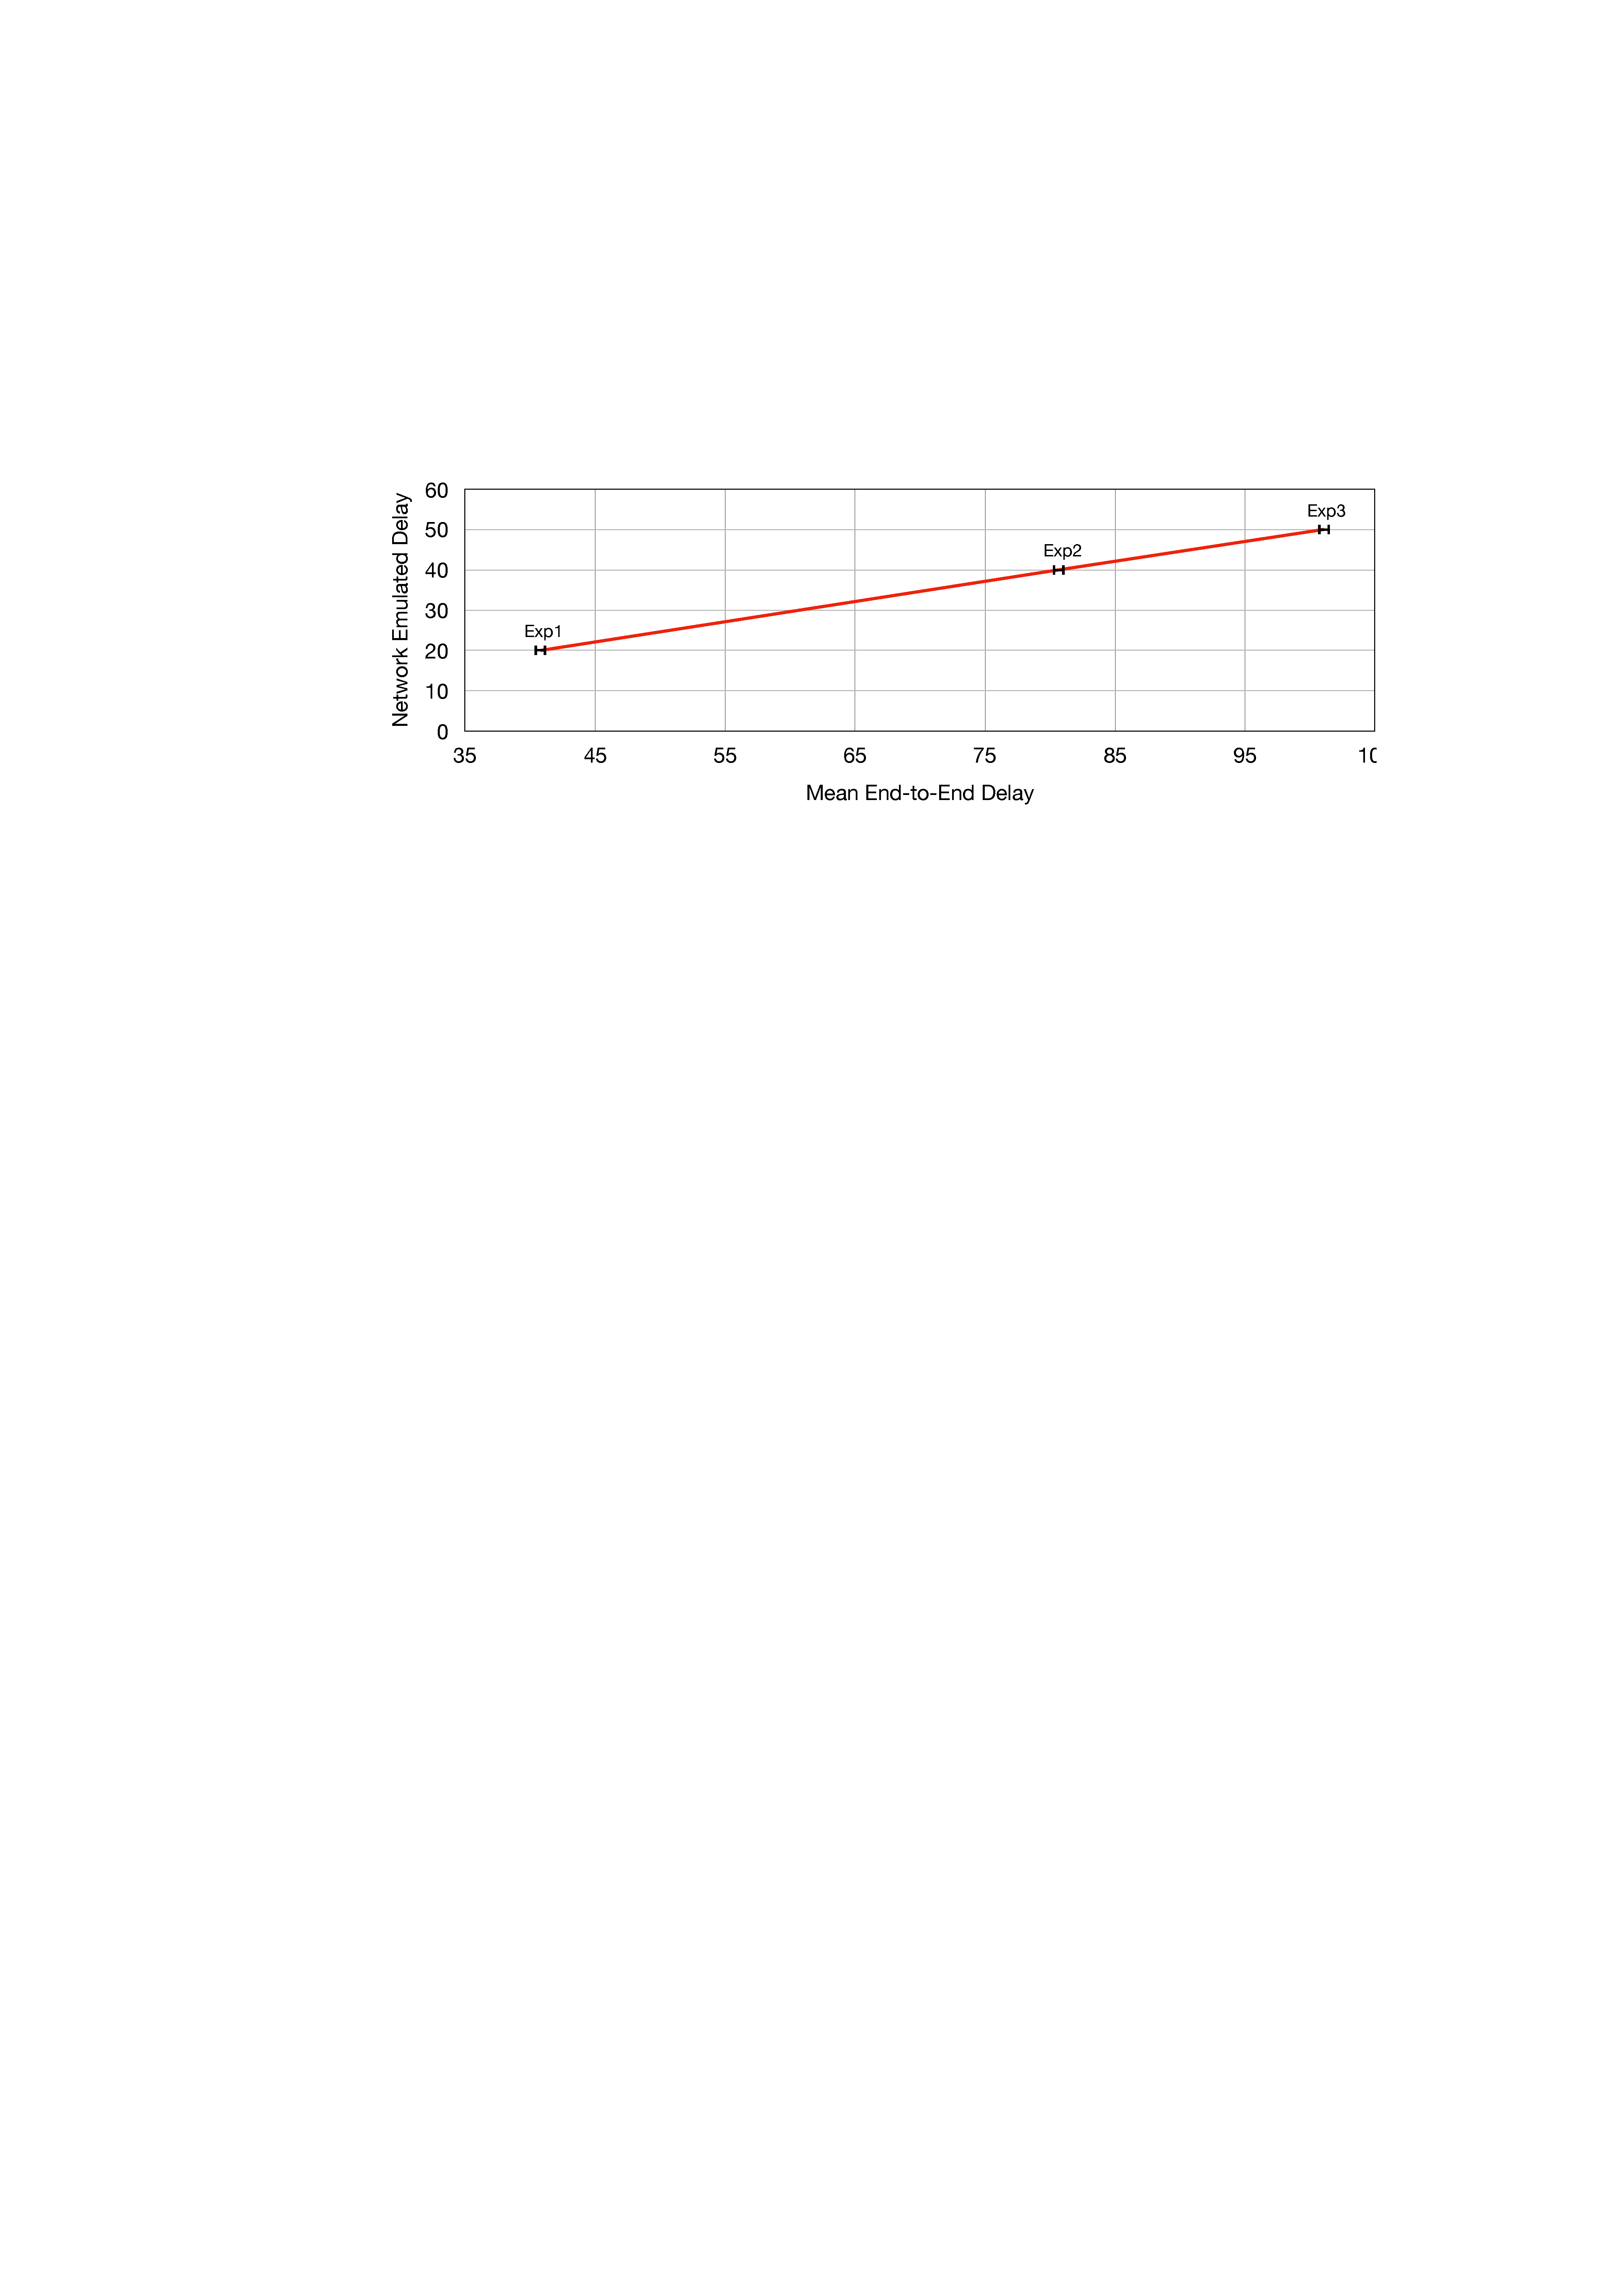
\includegraphics[width=\paperwidth]{exps.pdf}}
 %\caption{aaa}% do not put inside \makebox
 %\label{aaa}
%\end{figure*}


\end{document}
